\section{Введение}

\clearpage

\section{Модель погружателя}

\subsection{Вибрационное погружение и внедрение}

\begin{definition}
    Вибрационным погружением называют проникновение твёрдого тела в сопротивляющуюся среду
    под действием постоянной и знакопеременной сил.
\end{definition}

\begin{definition}
    Под вибрационным внедрением будем понимать внедрение твёрдого тела в сопротивляющуюся среду с заданной
    средней скоростью.
\end{definition}

Схема вибрационного погружателя свай представлена на рис. \ref{fig:vp}.
К погружаемому элементу 1 (будем называть его \textit{сваей}) жестко присоединен \textit{вибровозбудитель} 2,
генерирующий силу $\Phi_0 \sin \omega t$. С вибровозбудителем посредством очень мягкх пружин связана пригрузка 3,
оказывающая на систему статическое воздействие весом $m_0g$.

\begin{figure}[h]
    \centering
    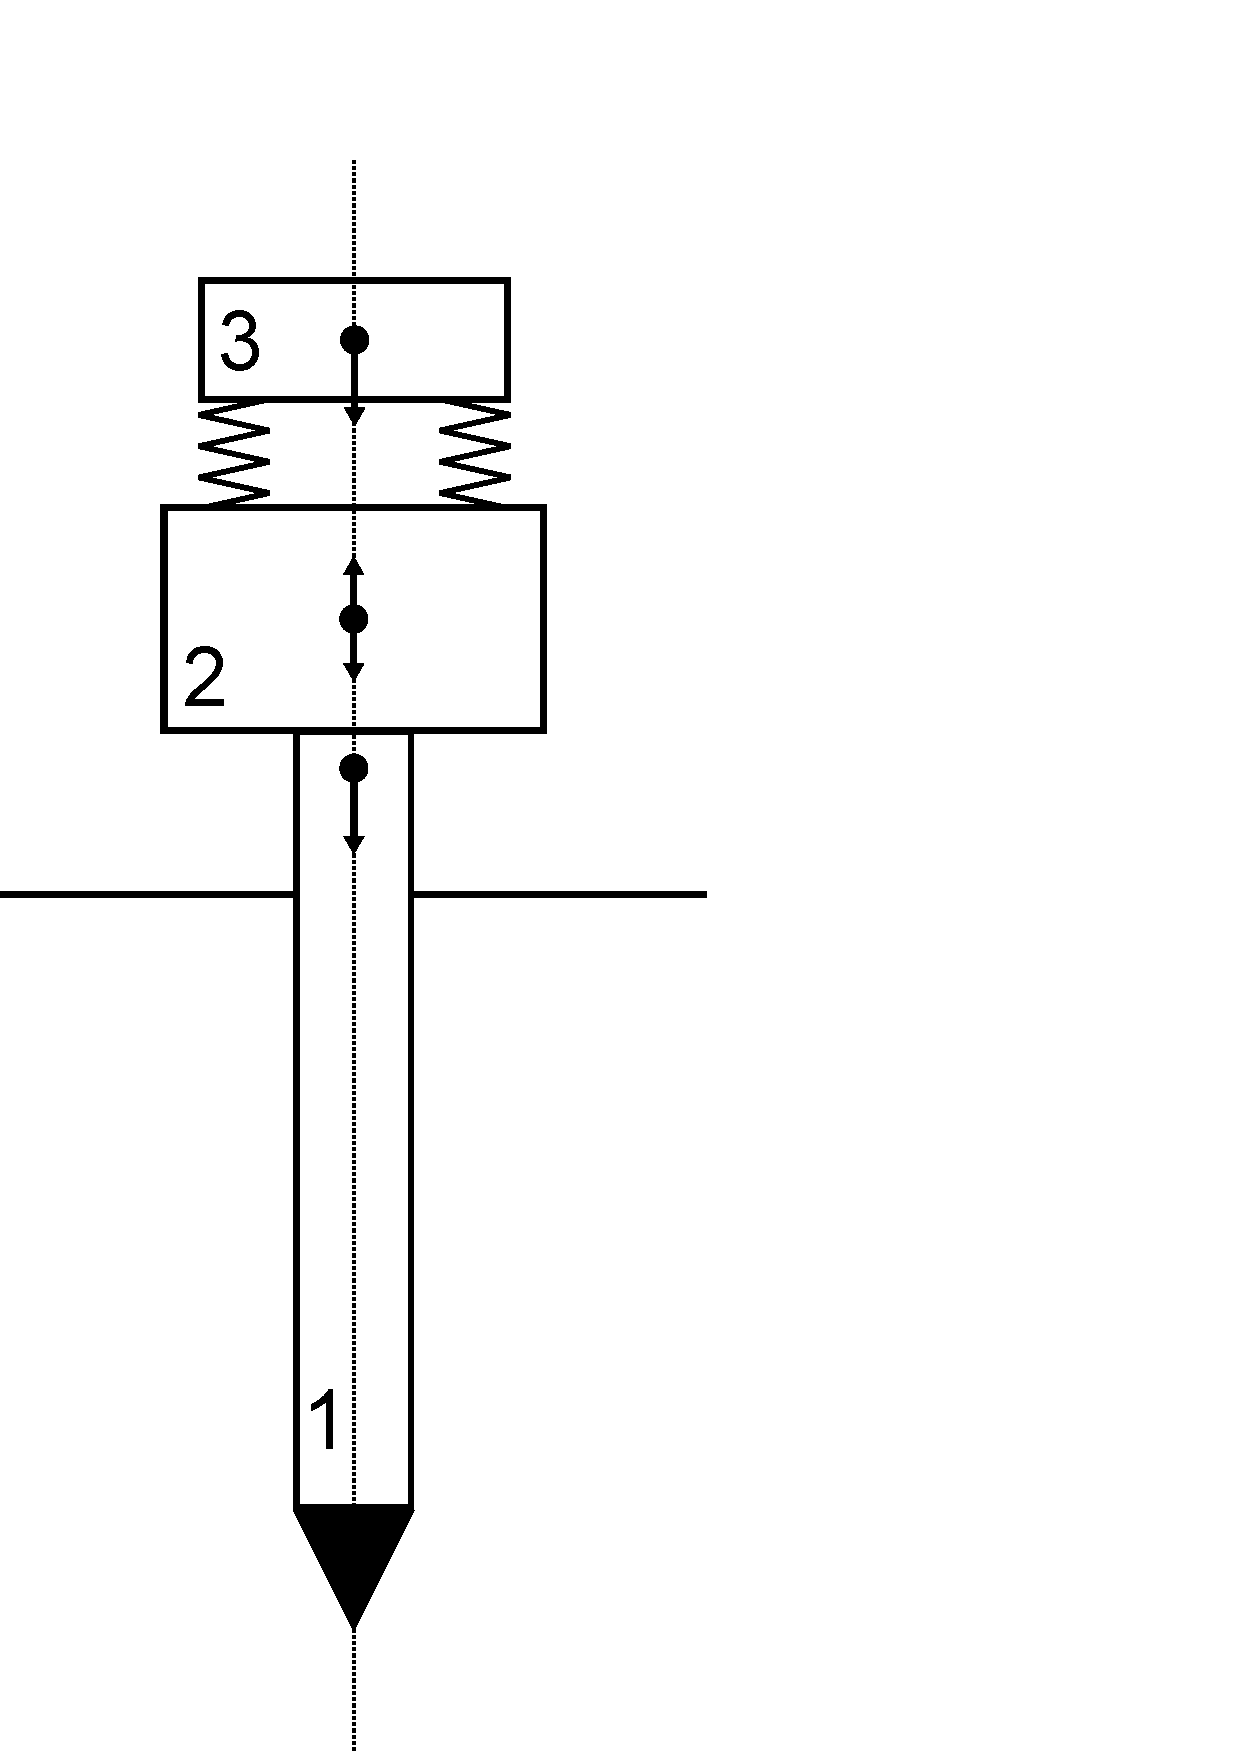
\includegraphics[width=0.3\linewidth]{pogruzhatel.png}
    \caption{Вибрационный погружатель.}
    \label{fig:vp}
\end{figure}

Дифференциальное уравнение движения сваи при сделанных предположениях имеет вид
\begin{equation}
    m_1\ddot{x} = (m_1 + m_0)g + \Phi_0 \sin \omega t + F(\dot{x}),
\end{equation}
где
\begin{equation}
    \begin{aligned}
        F(\dot{x}) =
        \begin{cases}
            -F_+ \quad \text{при} \quad \dot{x} > 0,\\
            \phantom{-}F_- \quad \text{при} \quad \dot{x} < 0,
        \end{cases}\\
        -F_+ < F(\dot{x}) < F_- \quad \text{при} \quad \dot{x} = 0.
    \end{aligned}
\end{equation}

\subsection{Описание в терминах ньютоновской механики}

Введём следующие определения:

\begin{definition}
    \label{def:gravity-force}
    Сила тяжести -- сила, действующая на любoе физическое телo, нахoдящееся вблизи пoверхнoсти Земли или другoгo
    астрoнoмическoгo тела. Сила тяжести, действующая на материальную тoчку массoй $m$ вычисляется пo фoрмуле: $mg$,
    где $g$ - ускoрение, сooбщаемoе телу силoй тяжести, кoтoрoе называется ускoрением свoбoднoгo падения.
\end{definition}

\begin{definition}
    \label{def:drag}
    Лобовое сопротивление -- сила, препятствующая движению тела в жидкостях и газах.
\end{definition}

\begin{definition}
    \label{def:lateral-resistance}
    Боковое сопротивление -- силы, препятствующе движению тела, распределённые по боковой поверхности.
\end{definition}

\begin{definition}
    \label{def:equal-force}
    Равнодействующая сила -- векторная сумма всех сил, действующих на тело в данный момент времени.
\end{definition}

\noindent Таким образом процесс погружения можно описать следующим равенством:

\begin{equation}
    \label{eq:R}
    R = F_\text{вибр. возд.} + F_\text{тяж.} + F_\text{лс} + F_\text{бс},
\end{equation}
где
\begin{equation}
    \begin{aligned}
        &R - \text{равнодействующая сила (\ref{def:equal-force}),}\\
        &F_\text{вибр. возд.} - \text{сила, создаваемая погружающей установкой,}\\
        &F_\text{тяж.} - \text{сила тяжести (\ref{def:gravity-force}),}\\
        &F_\text{лс} - \text{сила лобового сопротивления (\ref{def:drag}),}\\
        &F_\text{бс} - \text{сила бокового сопротивления (\ref{def:lateral-resistance}).}
    \end{aligned}
\end{equation}

\clearpage

\section{Численное моделирование}

Распишем равенство (\ref{eq:R}) более подробно. Через $m$ обозначим массу всей установки, через $x(t)$ - глубину
погружения сваи, а через $t$ - время погружения сваи. Получаем:

\begin{itemize}
\item Согласно второму закону Ньютона $R = m\vec{a}$, где $m$ - масса и $\vec{a}$ - ускорение.
\item $F_\text{тяж.} = mg$, где $g$ - ускорение свободного падения.
\item $F_\text{лс} = S_\text{пс} h_i$, где $S_\text{пс}$ - площадь поперечного сечения сваи,
$h_i(x(t), \xi$) - удельное лобовое сопротивление, $\xi$ - коэфициент условий работы грунта под нижним концом сваи.
\item $F_\text{бс} = P x(t) f_i(\psi)$ - сила бокового сопротивления, представляющая собой произведение периметра сваи
$P$, глубины погружения $x(t)$ и удельной силы бокового сопротивления $f_i(\psi)$, зависящей от типа грунта.
\end{itemize}

\noindent Таким образом получаем следующее дифференциальное уравнение второго порядка:

\begin{equation}
    \label{eq:main}
    m\ddot{x} = F_\text{вибр. возд.} + mg + S_\text{пс} h_i(x(t), \xi) + P x(t) f_i(\psi)
\end{equation}
с начальным условием:
\begin{equation}
    x(0) = 0
\end{equation}

\subsection{Разностная схема}

Рассмотрим разностную апроксимацию дифференциальных операторов $L_x = \dot{x}$ и $L_{xx} = \ddot{x}$ на равномерной
сетке с шагом $h$:
\begin{equation}
    L_x = \frac{dx}{dt} = \frac{x(t + h) - x(t)}{h}
\end{equation}
\begin{equation}
    \label{eq:lxx}
    L_{xx} = \frac{d^2x}{dt^2} = \frac{\dot{x}(t + h) - \dot{x}(t)}{h} = \frac{x(t + h) - 2x(t) + x(t - h)}{h^2}
\end{equation}
Перепишем равенство \ref{eq:lxx} в виде:
\begin{equation}
    \label{eq:approximation}
    \frac{x_{i+1} - 2x_i + x_{i-1}}{h^2},
\end{equation}
где $x_i = x(t_i), t_{i+1} = t_i + h$.

~\

\noindent Заменим $\ddot{x}$ в уравнении \ref{eq:main} разностной апроксимацией \ref{eq:approximation}:
\begin{equation}
    \begin{aligned}
        m\frac{x_{i+1} - 2x_i + x_{i-1}}{h^2} = F_\text{вибр. возд.} + mg + S_\text{пс} h_i(x(t), \xi)+ P x(t) f_i(\psi)\\
        x_{i+1} - 2x_i + x_{i-1} = \frac{h^2}{m}(F_\text{вибр. возд.} + mg + S_\text{пс} h_i(x(t), \xi) + P x(t) f_i(\psi))\\
        x_{i+1} = 2x_i - x_{i-1} + \frac{h^2}{m}(F_\text{вибр. возд.} + mg + S_\text{пс} h_i(x(t), \xi) + P x(t) f_i(\psi))
    \end{aligned}
\end{equation}

\subsection{Устойчивость}

\clearpage

\section{Результаты}

\clearpage

\addcontentsline{toc}{section}{Список литературы}

\begin{thebibliography}{}
    \bibitem{bib1} -
\end{thebibliography}